%%%%%%%%%%%%%%%%%%%%%%%%%%%%%%%%%%%%%%%%%
% SCRUM Guide v. 2011 - main latex file %
%%%%%%%%%%%%%%%%%%%%%%%%%%%%%%%%%%%%%%%%%

\documentclass[a4paper,12pt,oneside,titlepage]{article}

\usepackage[plainpages=false]{hyperref}
\usepackage[italian]{babel}
\usepackage[utf8]{inputenc}
\usepackage[T1]{fontenc}
\usepackage{textcomp}
\usepackage{color}
\usepackage[layout=modern]{./layout/advancedcoverpage}
\usepackage[scaled=.98]{helvet}

% hyperref setup to make linkable toc items 
\usepackage{hyperref}
\hypersetup{
    colorlinks,
    ps2pdf, 
    bookmarks=true, 
    bookmarksnumbered=false, 
    bookmarksopen=false, 
    linkcolor=black
    linktocpage,
    citecolor=black,
    filecolor=black,
    linkcolor=black,
    urlcolor=black
}

% Miscellaneous
\linespread{1.2}
\definecolor{Blue}{RGB}{63, 99, 141}
\definecolor{SteelBlue}{RGB}{70, 130, 180}
\definecolor{grey53}{RGB}{135, 135, 135}
\newcommand*\toccolor{
    \color{Blue}
}

% Format TOC
\usepackage[titles]{tocloft}
%\renewcommand{\cftsecleader}{\toccolor\cftdotfill{\cftsecdotsep}}
%\renewcommand*\cftsecpagefont{\toccolor}
\renewcommand*\cftsecfont{\fontsize{11}{13}\usefont{OT1}{phv}{c}{n}\selectfont}
\renewcommand*\cftsubsecfont{\fontsize{10}{12}\usefont{OT1}{phv}{c}{n}\selectfont}

% Header and Footer
\usepackage{fancyhdr}
\pagestyle{fancy}
\lhead{}
\chead{}
\rhead{}
\lfoot{\small{© 1991-2011 Ken Schwaber e Jeff Sutherland, All Rights Reserved}}
\cfoot{}
\rfoot{| \thepage} 
\renewcommand{\headrulewidth}{0pt}
\renewcommand{\footrulewidth}{0pt}

% Scrum logo
\usepackage[cc]{./layout/titlepic}
\usepackage{graphicx}
\titlepic{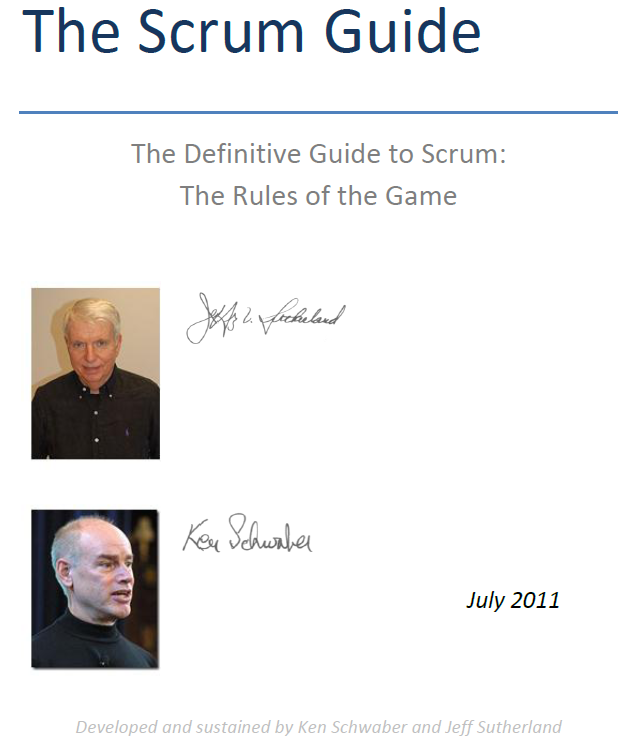
\includegraphics[width=\textwidth]{./images/scrum_coverpage.png}}

%%% Document
\begin{document}
    \date{}
    \title{}
    \maketitle
    \thispagestyle{fancy}
    \tocloftpagestyle{fancy}
    \tableofcontents
    \newpage
    \sffamily
	
    %%%%%%%%%%%%%%%%%%%%%%%%%%%%%%%%%%%%%%%%%%%%%%%%%%%%%%%%%%
% SECTION 1 : Scopo della Guida Scrum, Overview di Scrum %
%%%%%%%%%%%%%%%%%%%%%%%%%%%%%%%%%%%%%%%%%%%%%%%%%%%%%%%%%%

\section*{\color{Blue}{Scopo della Guida Scrum}}% (fold)
\label{sec:purpose}
\addcontentsline{toc}{section}{Scopo della Guida Scrum}
\pdfbookmark[1]{Scopo della Guida Scrum}{purpose}
Scrum \`e un framework per sviluppare e sostenere prodotti complessi. Questa guida contiene la definizione di Scrum. Questa 
definizione \`e costituita dai ruoli, gli eventi e gli artefatti di Scrum e le regole che li legano insieme. Ken Schwaber e Jeff 
Sutherland hanno sviluppato Scrum; la Guida Scrum \`e scritta e distribuita da loro.
% section purpose (end)

\section*{\color{Blue}{Overview di Scrum}}% (fold)
\label{sec:overview}
\addcontentsline{toc}{section}{Overview di Scrum}
\pdfbookmark[2]{Overview di Scrum}{overview}
Scrum (n): Un framework con il quale le persone possono affrontare complessi problemi di adattamento mentre in modo 
produttivo e creativo rilasciano prodotti dal pi\`u alto valore possibile. Scrum \`e:

\begin{itemize}
\item Leggero
\item Semplice da comprendere
\item Estremamente difficile da padroneggiare
\end{itemize}

Scrum \`e un framework di processo utilizzato a partire dai primi anni 1990 per gestire lo sviluppo di prodotti complessi. 
Scrum non \`e un processo o una tecnica per costruire prodotti ma piuttosto è un framework all'interno del quale \`e possibile 
utilizzare vari processi e tecniche. Scrum rende chiara l'efficacia relativa del tuo product management e delle pratiche di 
sviluppo usate in modo da poterle migliorare.

\subsection*{\color{SteelBlue}{Scrum Framework}}% (fold)
\label{sec:framework}
\addcontentsline{toc}{subsection}{Scrum Framework}
\pdfbookmark[3]{Scrum Framework}{framework}
Il framework Scrum \`e costituito dai Team Scrum e dai ruoli, eventi, artifatti e regole ad essi associati. Ogni componente del 
framewrok serve ad uno specifico scopo ed \`e essenziale per il successo e l'utilizzo di Scrum.
\newline
\\Strategie specifiche per l'utilizzo del framework Scrum variano e sono descritte altrove.
\newline
\\ Le regole di Scrum legano insieme gli eventi, i ruoli e gli artefatti governando le relazioni e le interazioni tra essi e 
sono descritte in tutto il corpo di questo documento.
% subsection framework (end)

%%section overview (end) % Scopo della Guida Scrum, Overview di Scrum
    %%%%%%%%%%%%%%%%%%%%%%%%%%%%%%%%%%%%%%%%%
% SECTION 2 : La Teoria di Scrum, Scrum	%
%%%%%%%%%%%%%%%%%%%%%%%%%%%%%%%%%%%%%%%%%

\section*{\color{Blue}{La Teoria di Scrum}}% (fold)
\label{sec:scrum_theory}
\addcontentsline{toc}{section}{La Teoria di Scrum}
\pdfbookmark[4]{La Teoria di Scrum}{scrum_theory}
Scrum si basa sulla teoria dei controlli empirici di processo o empirismo. L'empirismo afferma che la conoscenza deriva 
dall'esperienza e che le decisioni si basano su ci\`o che \`e noto. Scrum utilizza un metodo iterativo ed un approccio 
incrementale per ottimizzare la prevedibilit\`a ed il controllo del rischio. 
\newline

\\Sono tre i pilastri che sostengono ogni implementazione del controllo empirico di processo.

\subsection*{\color{SteelBlue}{Trasparenza}}% (fold)
\label{sec:transparency}
Gli aspetti significativi  del processo devono essere visibili ai responsabili del lavoro. La trasparenza richiede che quegli 
aspetti siano definiti da uno standard comune in modo tale che gli osservatori condividano una comune comprensione di ci\`o che 
viene visto.
\newline
\\Per esempio:
\begin{itemize}
	\item Un linguaggio comune di riferimento al processo deve essere condiviso da tutti i partecipanti; e,
	\item Una definizione comune di ``Fatto'' \footnote[1]{Vedere ``Definizione di Fatto'', pag. 
	      \pageref{sec:definition_of_done}} deve essere condivisa da chi esegue il lavoro e da chi deve accettare il lavoro.
\end{itemize}
% subsection transparency (end)

\subsection*{\color{SteelBlue}{Ispezione}}% (fold)
\label{sec:inspection}
Gli utenti di Scrum devono ispezionare frequentamente gli artefetti di Scrum e il progresso verso un obiettivo per rilevare le 
variazioni indesiderate. Le loro ispezioni non dovrebbero essere cos\`i frequenti da superare le soglie di tolleranza del 
processo alle ispezioni da rappresentare un'interruzione del lavoro. Le ispezioni sono pi\`u utili quando diligentemente 
eseguite da ispettori qualificati in corrispondenza del punto di lavoro.
% subsection inspection (end)

\subsection*{\color{SteelBlue}{Adattamento}}
\label{sec:adaptation}
Se chi  ispeziona verifica che uno o pi\`u aspetti del processo sono al di fuori dei limiti accettabili  e che il prodotto 
finale non potr\`a essere accettato, deve regolare il processo o il materiale lavorato.  La regolazione  deve essere  effettuata 
il  pi\`u rapidamente possibile per ridurre al minimo l'ulteriore scarto.

Scrum prescrive quattro occasioni formali per l'ispezione e l'adattamento, come descritto nella sezione ``Gli Eventi di Scrum'' 
di questo documento.

\begin{itemize}
     \item Scrum Planning Meeting
     \item Daily Scrum
     \item Sprint Review Meeting
     \item Sprint Retrospective
\end{itemize}
% subsection adaptation (end)

%% section scrum_theory (end)

\section*{\color{Blue}{Scrum}}% (fold)
\label{sec:scrum}
\addcontentsline{toc}{section}{Scrum}
\pdfbookmark[5]{Scrum}{scrum}
Scrum \`e un framework strutturato per supportare lo sviluppo di un prodotto complesso. Il framework Scrum \`e costituito dai 
Scrum Team e dai ruoli, gli eventi, gli artifatti e le regole ad essi associati. Ogni componente del framewrok serve ad uno 
specifico scopo ed \`e essenziale per il successo e l'utilizzo di Scrum. \newline

\\ Le regole di Scrum legano insieme gli eventi, i ruoli e gli artefatti governando le relazioni e le interazioni tra essi e 
sono descritte in tutto il corpo di questo documento.
%% section scrum (end) % La Teoria di Scrum, Scrum
    %%%%%%%%%%%%%%%%%%%%%%%%%%%%%
% SECTION 3 : Scrum Content %
%%%%%%%%%%%%%%%%%%%%%%%%%%%%%
\section*{\color{Blue}{LA SOSTANZA DI SCRUM}}
Il framework Scrum  \`e costituito da una serie  di
Scrum Team e dai ruoli ad essi associati: Time-Box, Artefatti e Regole.
I  Scrum Team sono  designati per  ottimizzare la  flessibilit\`a e  la produttivit\`a. Proprio per questo
sono auto-organizzati, cross-funzionali e lavorano su iterazioni.
Ogni Scrum Team ha tre ruoli: 

\begin{enumerate}
\item Scrum Master: si assicura che il processo \`e compreso e seguito;
\item Product Owner: responsabile di massimizzare il valore
del lavoro  che il  Team Scrum  fa; 
\item Team: fa  il lavoro. Il Team di
sviluppo ha  tutte le  competenze necessarie  per rispondere  alle esigenze  del
Product Owner e per  produrre, entro  la fine  dello Sprint, una
porzione potenzialmente rilasciabile di prodotto.
\end{enumerate}

Scrum impiega intervalli  di tempo per creare regolarit\`a.  Gli elementi che appartengono a questo intervallo temporale sono:
\begin{itemize}
\item Release  Planning  Meeting 
\item Sprint Planning  Meeting
\item Sprint
\item Daily Scrum Meeting
\item Sprint Review
\item Sprint Retrospective
\end{itemize}

Il cuore di Scrum \`e lo \textbf{Sprint}, cio\`e una iterazione di un mese o meno, coerente per
tutta la lunghezza del progetto.

Tutti gli sprint utilizzano  lo stesso framework Scrum  e tutti
gli sprint  forniscono un  incremento del  prodotto finale  che \`e potenzialmente
rilasciabile.  Uno  Sprint inizia  immediatamente  dopo l'altro.

Scrum  impiega principalmente quattro artefatti:\begin{itemize}
\item[-] Product Backlog: \`e l'elenco prioritario di tutto ci\`o che potrebbe essere necessario al prodotto;
\item[-] Sprint Backlog: \`e la lista di compiti per trasformare  l'arretrato di prodotto per uno Sprint in
un incremento  potenzialmente rilasciabile;
\item[-] Burndown: \`e la misura del Product Backlog residuo nel corso del tempo;
\item[-] Release Burndown: \`e la misura del Product Backlog rimanente  al tempo del piano di rilascio;
\item[-] Sprint Burndown: \`e la  misura degli elementi restanti dello Sprint Backlog
nel tempo  di uno  Sprint.
\end{itemize}

Le regole legano insieme i time-boxes, i ruoli e gli artefatti e vengono descritte in questo documento.
Per  esempio, \`e regola  che solo  i membri  del Team  Scrum -  le persone
impegnate a  trasformare l'arretrato  del prodotto  in un  incremento -  possono
parlare durante un Daily Scrum Meeting. Daremo dei ''TIP'' - Suggerimenti per descrivere
le modalit\`a di implementazione di  Scrum che non sono regole.
\vspace{0.4cm}

\fbox{
\begin{minipage}{0.9\textwidth}
\begin{large}TIP\end{large}\\
Quando le regole non sono precise, chi usa Scrum si aspetta di capire cosa fare. Non \`e importante cercare una soluzione perfetta, perch\`e il problema di solito cambia rapidamente. Al contrario, bisogna provare qualcosa e capirne il funzionamento. I meccanismi di natura empirica di ispezione-adeguamento di Scrum ci guideranno.
\end{minipage}
} % Scrum Team
    %%%%%%%%%%%%%%%%%%%%%%%%%%%
% SECTION 4 : Scrum Roles %
%%%%%%%%%%%%%%%%%%%%%%%%%%%
\newpage
\section*{I RUOLI}
\label{sec:roles}

\subsection*{LO SCRUM MASTER}
\label{sec:scrummaster}
TODO

\subsection*{IL PRODUCT OWNER}
\label{sec:productowner}
TODO

\subsection*{IL TEAM}
\label{sec:team}
TODO % Gli Eventi di Scrum
    %%%%%%%%%%%%%%%%%%%%%%%%%%%%%%%%%%%%%%
% SECTION 5 : Gli Artefatti di Scrum %
%%%%%%%%%%%%%%%%%%%%%%%%%%%%%%%%%%%%%%

\section*{\color{Blue}{Gli Artefatti di Scrum}}
\label{sec:artifacts}
\addcontentsline{toc}{section}{Gli Artefatti di Scrum}
\pdfbookmark[16]{Gli Artefatti di Scrum}{artifacts}
Gli artefatti di Scrum rappresentano il lavoro o il valore in diversi modi tale da risultare utili a fornire trasparenza e 
opportunit\`a di ispezione e adattamento. Gli artefatti definiti da Scrum sono specificatamente progettati per massimizzare la 
trasparenza delle informazioni chiave necessarie ad assicurare ai Team Scrum il successo nella realizzazione di un Incremento 
``Fatto''.

\subsection*{\color{SteelBlue}{Product Backlog}}
\label{sec:product_backlog}
\addcontentsline{toc}{subsection}{Product Backlog}
\pdfbookmark[17]{Product Backlog}{product_backlog}
Il Product Backlog \`e un elenco ordinato di tutto ciò che potrebbe essere necessario al prodotto ed \`e l'unica fonte di 
requisiti per le modifiche da apportare al prodotto. Il Product Owner \`e il responsabile del Product Backlog, compreso il suo 
contenuto, la sua disponibilità e l'ordinamento dei suoi elementi. \newline
\\Un Product Backlog non \`e mai completo. Il suo primo sviluppo definisce solo i requisiti inizialmente conosciuti e 
meglio compresi. Il Product Backlog evolve come il prodotto e l'ambiente in cui verrà utilizzato. \`E dinamico e cambia 
continuamente per identificare ci\`o che serve al prodotto per risultare adeguato, competitivo e utile. Finch\`e esiste un 
prodotto, esiste anche un Product Backlog. \newline
\\Il Product Backlog elenca tutte le caratteristiche, le funzioni, i requisiti, le migliorie e le correzioni che costituiscono 
le modifiche al prodotto nelle future versioni. I suoi elementi hanno una descrizione, un ordine ed una stima. \newline
\\ \`E spesso ordinato per valore, per rischio, per priorità e necessità. L'ordinamento dall'alto verso il basso degli 
elementi del Product Backlog guida le attività di sviluppo. Pi\`u alto \`e l'ordine, pi\`u la voce del Product Backlog \`e 
stata considerata ed il consenso su di essa e sul suo valore \`e maggiore. \newline
\\Gli elementi con ordine superiore sono pi\`u chiari e meglio dettagliati rispetto a quelli con ordine inferiore. Le stime 
risultano pi\`u precise e si basano sulla maggiore chiarezza e maggior numero di dettagli; minore è l'ordine e minore \`e il 
livello di dettagli. Gli elementi del Product Backlog che occuperanno il Team di Sviluppo per il prossimo Sprint sono a grana 
fine, dopo essere stati suddivisi in modo tale che ogni elemento pu\`o essere considerato un ``Fatto'' entro i tempi dello 
Sprint. Gli elementi del Product Backlog che possono essere ``Fatti'' dal Team di Sviluppo durante un Sprint sono considerati 
``pronti'' o ``perseguibili'' per essere selezionati durante l'incontro di Sprint Planning. \newline
\\Quando un prodotto viene utilizzato, acquista valore e il mercato fornisce un feedback, il Product Backlog diventa un elenco 
pi\`u completo ed  esaustivo. I requisiti non smettono mai di cambiare, cos\`i il Product Backlog \`e un artefatto vivente. I 
cambiamenti nei requisiti di business, le condizioni di mercato o la tecnologia possono causare cambiamenti nel Product 
Backlog. \newline
\\Numerosi Team Scrum si trovano spesso a lavorare sullo stesso prodotto. Un Product Backlog \`e usato per descrivere il lavoro 
imminente sul prodotto. \`E poi impiegato un backlog degli attributi del prodotto che raggruppa gli elementi .\newline
\\ Il grooming del Product Backlog \`e l'atto di aggiungere dettagli, stime e ordine agli elementi del Product Backlog. Questo 
\`e un processo continuo in cui il Product Owner e il Team di Sviluppo collaborano sui dettagli degli elementi del Product 
Backlog. Durante il grooming del Product Backlog, i suoi elementi vengono riesaminati e rivisti. Tuttavia, essi possono essere 
aggiornati in qualsiasi momento dal Product Owner o a discrezione del Product Owner. \newline
\\Il grooming \`e un'attivit\`a  part-time durante uno Sprint tra il Product Owner ed il Team di Sviluppo. Spesso il Team di 
Sviluppo ha la conoscenza di dominio per eseguire il grooming stesso. \`E il Team Scrum che decide come e quando fare grooming. 
L'attivit\`a di grooming consuma solitamente non pi\`u del 10\% della capacità del Team di Sviluppo. \newline
\\Il Team di Sviluppo \`e responsabile di tutte le stime. Il Product Owner pu\`o influenzare il Team aiutando a capire e 
selezionare i trade-off, ma chi eseguer\`a il lavoro fa la stima finale.

\subsubsection*{\color{SteelBlue}{Monitorare i Progressi verso un Obiettivo}} % (fold)
\label{ssub:monitoring_progress_toward_a_great}
In qualsiasi momento il rimanente lavoro totale per raggiungere un obiettivo pu\`o essere sommato. Il 
Product Owner traccia il lavoro totale almeno ad ogni Sprint Review. Confronta questa cifra con il 
lavoro rimanente delle precedenti Sprint Review e valuta i progressi verso il completamento dei 
lavori per raggiungere l'obiettivo previsto al tempo desiderato. Queste informazioni vengono rese trasparenti a 
tutti gli stakeholder.\newline
\\Scrum non considera il tempo impiegato per lavorare sugli elementi del Product Backlog. Il lavoro 
rimanente e la data sono le uniche  variabili di interesse. \newline
\\Diversi trend burndown, burnup e altre pratiche proiettive sono state utilizzate per prevedere il 
progresso. Queste si sono rilevate utili. Tuttavia, queste tecniche non sostituiscono l'importanza 
dell'empirismo. In ambienti complessi, cosa accadr\`a \`e sconosciuto, solo ci\`o che \`e successo pu\`o 
essere utilizzato in un futuro processo decisionale.
% subsubsection monitoring_progress_toward_a_great (end)

% subsection product_backlog (end)

\subsection*{\color{SteelBlue}{Sprint Backlog}}
\label{sec:sprint_backlog}
\addcontentsline{toc}{subsection}{Sprint Backlog}
\pdfbookmark[18]{Sprint Backlog}{sprint_backlog}
Lo Sprint Backlog \`e l'insieme delle voci selezionate dal Product Backlog per lo Sprint, 
pi\`u un piano per la distribuzione dell'incremento di prodotto e la realizzazione 
dell'obiettivo di Sprint. Lo Sprint Backlog rappresenta una previsione del Team di 
Sviluppo circa la funzionalità che rappresenter\`a  l'incremento successivo ed il lavoro 
necessario per rilasciare questa funzionalit\`a. \newline
\\ Lo Sprint Backlog definisce il lavoro che il Team di Sviluppo eseguir\`a per 
trasformare gli elementi del Product Backlog in un incremento ``Fatto''. Lo Sprint Backlog rende visibile tutto il 
lavoro che il Team di Sviluppo identifica come necessario per soddisfare l'obiettivo di Sprint. \newline
\\Lo Sprint Backlog \`e un piano con dettagli sufficienti affinch\`e i cambiamenti in atto 
possono essere compresi nel Daily Scrum. Il Team di Sviluppo modifica lo Sprint Backlog 
durante tutto lo Sprint e lo Sprint Backlog emerge durante lo Sprint. Questa emergenza si 
verifica quando il Team di Sviluppo opera attraverso il piano e viene a conoscenza di 
pi\`u dettagli sul lavoro necessario per raggiungere l'obiettivo di Sprint. \newline
\\Quando del nuovo lavoro risulta necessario, il Team di Sviluppo lo aggiunge allo Sprint 
Backlog. Poich\`e il lavoro viene eseguito o completato, il rimanente lavoro stimato viene 
aggiornato. Quando gli elementi del piano sono ritenute inutili, vengono rimossi. Solo il 
Team di Sviluppo pu\`o cambiare il suo Sprint Backlog nel corso di uno Sprint. Lo Sprint 
Backlog ha una grande visibilit\`a, \`e un'immagine in tempo reale del lavoro che il Team 
di Sviluppo prevede di realizzare durante lo Sprint; appartiene soltanto al Team di Sviluppo.

\subsubsection*{\color{SteelBlue}{Monitorare i Progressi dello Sprint}} % (fold)
\label{ssub:monitoring_sprint_progress}
In qualsiasi istante temporale durante uno Sprint, il rimanente lavoro totale del Product Backlog 
pu\`o essere sintetizzato. Il Team di Sviluppo traccia il rimanente lavoro totale quantomeno 
ad ogni Daily Scrum. Traccia queste somme giornalmente e progetta la probabilit\`a di 
raggiungere l'obiettivo dello Sprint. Tracciando il lavoro rimanente per tutto lo Sprint, 
il Team di Sviluppo \`e in grado di gestire il proprio progresso. \newline
\\Scrum non considera il tempo impiegato per lavorare sugli elementi dello Sprint Backlog. 
Il lavoro rimanente e la data sono le uniche variabili di interesse. 
% subsubsection monitoring_sprint_progress (end)

% subsection sprint_backlog (end)

\subsection*{\color{SteelBlue}{Incremento}}
\label{sec:increment}
\addcontentsline{toc}{subsection}{Incremento}
\pdfbookmark[19]{Incremento}{increment}
L'incremento \`e la somma di tutti gli elementi del Product Backlog completati durante uno 
Sprint e tutti gli Sprint precedenti. Alla fine di uno Sprint, il nuovo Incremento deve 
essere ``Fatto'', il che significa che deve essere utilizzabile e deve incontrare la 
definizione di ``Fatto'' data dal Team Scrum. Deve essere utilizzabile indipendentemente dal 
fatto che il Product Owner decide di rilasciarlo realmente.
% subsection increment (end)

%% section artifacts (end)
 % Gli Artefatti di Scrum
    %%%%%%%%%%%%%%%%%%%%%%%%%%%%%%%
% SECTION 6 : Scrum Artifacts %
%%%%%%%%%%%%%%%%%%%%%%%%%%%%%%%
\section*{\color{Blue}{ARTEFATTI}}
\label{sec:artifacts}
Gli artefatti includono il Product Backlog, il Release Burndown, lo Sprint Backlog e lo Sprint Burndown.

\subsection*{\color{Blue}{PRODUCT BACKLOG E RELEASE BURNDOWN}}
\label{sec:productbacklog}
I requisiti per il prodotto che il Team (s) \`e in via di sviluppo sono elencati nella Backlog prodotto. Il
proprietario del prodotto \`e responsabile per l'arretrato del prodotto, il suo contenuto, la sua disponibilit\`a, e la
sua priorit\`a. Backlog prodotto non \`e mai completa. Il taglio iniziale di sviluppo che prevede solo la inizialmente
conosciuto e meglio comprendere i requisiti. Il portafoglio ordini del prodotto si evolve come il prodotto e l'ambiente
in cui verr\`a utilizzato evolve. L'arretrato \`e dinamico, nel senso che cambia continuamente di individuare ci\`o che
il prodotto deve essere adeguato, competitivo e utile. Finch\`e un prodotto esiste, esiste anche Backlog prodotto.\\
\linebreak 
Il portafoglio ordini del prodotto rappresenta tutto il necessario per sviluppare e lanciare un prodotto di
successo. Si tratta di un elenco di tutte le caratteristiche, le funzioni, le tecnologie, miglioramenti e correzioni di
bug, che costituiscono le modifiche che saranno apportate al prodotto per le versioni future. Oggetti Backlog Prodotto
hanno gli attributi di una descrizione, la priorit\`a, e stima. La priorit\`a \`e guidato da rischi, il valore, e la
necessit\`a. Ci sono molte tecniche per la valutazione di tali attributi.

\tip{da tradurre}

Backlog prodotto \`e ordinato secondo una priorit\`a. Backlog Top Product priorit\`a unit\`a le attivit\`a di sviluppo
immediato. Maggiore \`e la priorit\`a pi\`u urgente \`e, pi\`u si \`e pensato, e il consenso pi\`u c'\`e per quanto
riguarda il suo valore. Backlog priorit\`a pi\`u alt\`a \`e pi\`u chiaro e ha informazioni pi\`u dettagliate rispetto a
backlog priorit\`a pi\`u bassa. Meglio le stime sono fatte in base al maggior chiarezza e dettaglio maggiore. Pi\`u
bassa \`e la priorit\`a, tanto meno i dettagli, fino a quando non riesce a malapena a distinguere il prodotto.\\
\linebreak

Come un prodotto viene utilizzato, in quanto il suo valore aumenta, e come il mercato fornisce un feedback, arretrato
del prodotto emerge in una lista pi\`u ampia e completa. Requisiti non si fermano mai cambiare. Il Product Backlog \`e
un documento vivo. Cambiamenti nei requisiti di business, le condizioni di mercato, la tecnologia, e il personale
causare modifiche nel backlog prodotto. Per ridurre al minimo le rilavorazioni, solo gli elementi pi\`u alta priorit\`a
devono essere dettagliate fuori. Le voci Backlog prodotto che si occupano delle squadre per il prossimo sprint diversi
sono a grana fine, essendo stato scomposto in modo che ogni elemento pu\`o essere effettuata entro la durata della
Sprint.

\tip{da tradurre}

Multiple squadre Scrum spesso lavorano insieme su uno stesso prodotto. Un backlog di prodotto \`e utilizzato per
descrivere i lavori imminenti sul Prodotto. Un attributo Backlog prodotto che gli elementi dei gruppi viene poi
impiegato. Raggruppamento si pu\`o verificare dal set di funzionalit\`a, la tecnologia, o l'architettura, ed \`e spesso
usato come un modo per organizzare il lavoro con Scrum Team.

\tip{da tradurre}

Il grafico Release Burndown registra la somma di Portafoglio ordini residuo stimato lo sforzo prodotto nel tempo. Lo
sforzo \`e stimato in qualsiasi unit\`a di lavoro del Team Scrum e l'organizzazione sono decise. Le unit\`a di tempo
sono di solito Sprint.\\ 
\linebreak

Stime voce del Product Backlog sono calcolati inizialmente durante la Release Planning, e, successivamente, come
vengono creati. Durante Backlog prodotto grooming sono riesaminato e rivisto. Tuttavia, essi possono essere aggiornati
in qualsiasi momento. Il Team \`e responsabile di tutte le stime. Il Product Owner pu\`o influenzare la squadra,
aiutando a capire e selezionare trade-off, ma la stima finale \`e fatta dal team. Il Product Owner mantiene un elenco
aggiornato dei prodotti Backlog Backlog Release Burndown Posted in ogni momento. La linea di tendenza si possono trarre
sulla base del cambiamento di lavoro rimanente.

\tip{da tradurre}

\subsection*{\color{Blue}{SPRINT BACKLOG E SPRINT BURNDOWN}}
\label{sec:sprintbacklog}
Lo Sprint Backlog comprende i compiti del team esegue a sua volta elementi Backlog prodotto in un ''fatto'' di
incremento. Molti sono sviluppate durante la Sprint Planning Meeting. \`E tutto il lavoro che il team identifica come
necessario per soddisfare l'obiettivo Sprint. Oggetti Backlog Sprint deve essere scomposto. La decomposizione \`e
sufficiente modo che le modifiche in corso pu\`o essere compreso nel Daily Scrum.

\tip{da tradurre}

Il team di modifica Backlog Sprint tutta la Sprint, cos\`i come Backlog Sprint emergenti durante la Sprint. Come si
arriva in singole attivit\`a, si pu\`o scoprire che i compiti pi\`u o meno sono necessari, o che un determinato compito
sar\`a pi\`u o meno tempo di quanto fosse stato previsto. Come nuovo lavoro \`e necessario, il Team si aggiunge al
residuo Sprint. Come compiti sono manipolate o completati, le ore di lavoro stimato rimanente per ogni compito \`e
aggiornato. Quando le attivit\`a sono ritenute inutili, che vengono rimossi. Solo il team pu\`o cambiare il suo corso
di uno Sprint Backlog. Solo il team possono modificare i contenuti o le stime. Lo Sprint Backlog ha una grande
visibilit\`a, immagine in tempo reale del lavoro che il team ha in programma di realizzare nel corso della Sprint, ed
appartiene esclusivamente al team.\\ 
\linebreak

Backlog Sprint Burndown \`e un grafico della quantit\`a di lavoro Portafoglio ordini residuo in un Sprint Sprint
attraverso il tempo nella Sprint. Per creare questo grafico, determinare quanto lavoro resta sommando il ritardo stime
ogni giorno della Sprint. La quantit\`a di lavoro rimanente per un Sprint \`e la somma del lavoro rimanente per tutti
Backlog Sprint. Tenere traccia di queste somme di giorno e li usa per creare un grafico che mostra i restanti lavori
nel corso del tempo. Tracciando una linea attraverso i punti del grafico, il team in grado di gestire i suoi progressi
nel completamento di un lavoro di Sprint. Durata non \`e considerato in Scrum. Restanti lavori \`e la data sono le sole
variabili di interesse.\\ 
\linebreak 

Una delle regole Scrum appartiene alla fine di ogni Sprint, che \`e quello di fornire incrementi di funzionalit\`a
potenzialmente rilasciabile che aderisca ad una definizione operativa di ''fatto''.

\tip{da tradurre}

\subsection*{\color{Blue}{FATTO}}
\label{sec:done}
Scrum richiede squadre di costruire un incremento delle funzionalit\`a del prodotto ogni Sprint. Tale incremento deve
essere potenzialmente rilasciabile, per il prodotto proprietario pu\`o scegliere di applicare subito la funzionalit\`a.
Per fare ci\`o, l'incremento deve essere una fetta completa del prodotto. Essa deve essere ''fatto.'' Ogni incremento
dovrebbe essere a tutti gli additivi incrementi precedenti e testato, assicurando che tutti incrementi lavorare
insieme.

\tip{da tradurre}

Nello sviluppo del prodotto, affermando che la funzionalit\`a \`e fatto potrebbe portare qualcuno a ritenere che, in
almeno pulito codice, il refactoring, unit test, costruito e testato l'accettazione. Qualcun altro potrebbe supporre
solo che il codice \`e stato costruito. Se tutti non sa che la definizione di ''fatto'' \`e, gli altri due le gambe di
controllo del processo empirico non funzionano. Quando qualcuno descrive come fare qualcosa, ognuno deve capire cosa si
intende fare.\\
\linebreak

Fatto definisce ci\`o che il team intende quando si impegna a ''fare'' un elemento di backlog prodotto in uno sprint.
Alcuni prodotti non contengono la documentazione, quindi la definizione di ''fatto'' non comprende la documentazione. A
completamente ''fatto'' incremento include tutte le analisi, progettazione, refactoring, programmazione, documentazione
e analisi per l'incremento e tutti gli elementi backlog prodotto in incremento. Test comprende unit\`a, di sistema,
l'utente, e di regressione, così come non le prove funzionali, come le prestazioni, stabilit\`a, sicurezza e
integrazione. Fatto include qualsiasi internazionalizzazione. Alcune squadre non sono ancora in grado di comprendere
tutto il necessario per l'esecuzione nella loro definizione di fatto. Questo deve essere chiaro per il proprietario del
prodotto. Questo lavoro rimanente dovr\`a essere fatta prima che il prodotto pu\`o essere implementato e utilizzato. % Definizione di “Fatto”
    %%%%%%%%%%%%%%%%%%%%%%%%%%%%%%%%%%%%%%%%%%%%%%%%%%%%%%
% SECTION 7 : Conclusioni, Ringraziamenti, Revisioni %
%%%%%%%%%%%%%%%%%%%%%%%%%%%%%%%%%%%%%%%%%%%%%%%%%%%%%%
\newpage
\section*{\color{Blue}{Ringraziamenti}}
\label{sec:acknowledgements}

\subsection*{\color{SteelBlue}{Persone}}
\label{sec:people}
Delle migliaia di persone che hanno contribuito a Scrum, dovremmo individuare coloro che hanno contribuito nei suoi
primi dieci anni. Prima c'erano Jeff Sutherland, in collaborazione con Jeff McKenna, e Ken Schwaber con Mike Smith e
Chris Martin. Molti altri hanno contribuito negli anni successivi e senza il loro aiuto non sarebbe stato possibile ridefinire Scrum in ci\`o che oggi \`e. David Starr ha approfondito e fornito le competenze editoriali per la formulazione di questa versione della Guida a Scrum.

\subsection*{\color{SteelBlue}{Storia}}
\label{sec:history}
Ken Schwaber e Jeff Sutherland hanno presentato per la prima volta Scrum alla conferenza OOPSLA del 1995. Questa presentazione ha essenzialemente documentato ci\`o che Ken e Jeff avevano appreso negli anni precedenti applicando Scrum.

La storia di Scrum pu\`o gi\`a essere considerata lunga. Per ricordare i primi posti in cui \`e stato richiesto ed adottato, onoriamo Individual, Inc. Fidelity Investments, e IDX (oggi GE Medical).

\newpage
\section*{\color{Blue}{Revisioni}}
\label{sec:revisions}
Questa versione di luglio 2011 della Guida a Scrum è diversa dalla precedente di febbraio 2010. In particolare abbiamo cercato di rimuovere le tecniche o le best practices dal nucleo di Scrum. Questi variano a seconda della circostanza. Inizieremo pi\`u tardi con un compedio di ``Best Practices'' per offrire alcune delle nostre esperienze.

La Guida a Scrum Guida documenta come Scrum \`e stato sviluppato e sostenuto da pi\`u di venti anni da Jeff Sutherland e Ken Schwaber. Altre fonti forniscono modelli, processi e idee sulle pratiche, le agevolazioni e gli strumenti che completano il framewok Scrum. Queste ottimizzano la produttività, il valore, la creatività e l'orgoglio.

Le note di rilascio che coprono le seguenti differenze tra questa e la versione di Febbraio 2010 saranno pubblicate altrove, comprese le discussioni su:

\begin{enumerate}
 	\item Release Planning
	\item Release Burndown
	\item Sprint Backlog
	\item Product e Sprint Backlog Burndown
	\item Team (per Development Team)
	\item Maiali e Polli...la tradizione di Scrum
	\item Ordinati invece che prioritizzati 
\end{enumerate}

\newpage
\section*{\color{Blue}{Traduzione}}
\label{sec:translation}
Questo documento \`e stato tradotto dalla versione originale inglese di Ken Schwaber e Jeff Sutherland. Hanno contribuito a realizzare la traduzione Carlo Beschi e Mirco Veltri.

\section*{\color{Blue}{Note alla versione italiana}}
\label{sec:transnotes}
I sorgenti della traduzione sono disponibili sul repository \htmladdnormallink{GitHub}{http://github.com/indaco/scrumguide-ita}. 
Sentitevi liberi di contattare i traduttori per segnalare errori o semplicemente per lasciare un feedback. Grazie.
 % Conclusioni, Ringraziamenti, Revisioni
\end{document}